\subsection{Approximating the Step Response}

Unfortunately, it is not  possible  to directly calculate appropriate values for
$n$, $T$ and  $r$,  however,  what equations \ref{eq:ptn}, \ref{eq:hudzovic} and
\ref{eq:sani}  allow  us  to  do  now  is  calculate an infinite number of  step
responses of arbitrary order  (while  maintaining  a  constant  number  of input
arguments, thanks to the  function  $T_k(r)$),  characterise  the response using
equations   \ref{eq:tu_tg}   or   \ref{eq:t10_t50_t90}   (i.e.   determine   its
``complexity''), and perform a reverse  lookup  on  those  results  to  find the
parameters  $n$,  $T$, and $r$. In practice, it is sufficient to calculate about
50 step responses for each order and interpolate between those values when doing
the lookup, as will be shown in this paper.

As discussed earlier, a remarkable  observation  is  that the parameters $r$ and
$n$ are independent of time and amplitude (and offset); that is,  the normalised
step response does not change its  shape when the parameter $T$ is changed. This
is fantastic,  because  it  allows  us  to eliminate a dimension from the lookup
table.

If we set $T=1$, $K_s=1$ and $y_0=0$, we  can  use  equations  \ref{eq:ptn}  and
\ref{eq:hudzovic} to  calculate  a  series  of  transfer  functions  $G_n(s,r)$,
calculate  their  time  domain  step  responses   $g_{r,n}(t)$,   and  calculate
$g_{T_u/T_g}$ and $g_{1/T_g}$ for each step response.

Thus, $g_{T_u/T_g}$ and $g_{1/T_g}$ can both be expressed as  functions  of  $r$
and $n$:

\begin{align}
    g_{T_u/T_g} = g_{T_u/T_g}(r, n) \\
    g_{1/T_g}  =  g_{1/T_g}(r,n)
\end{align}

\begin{figure}
    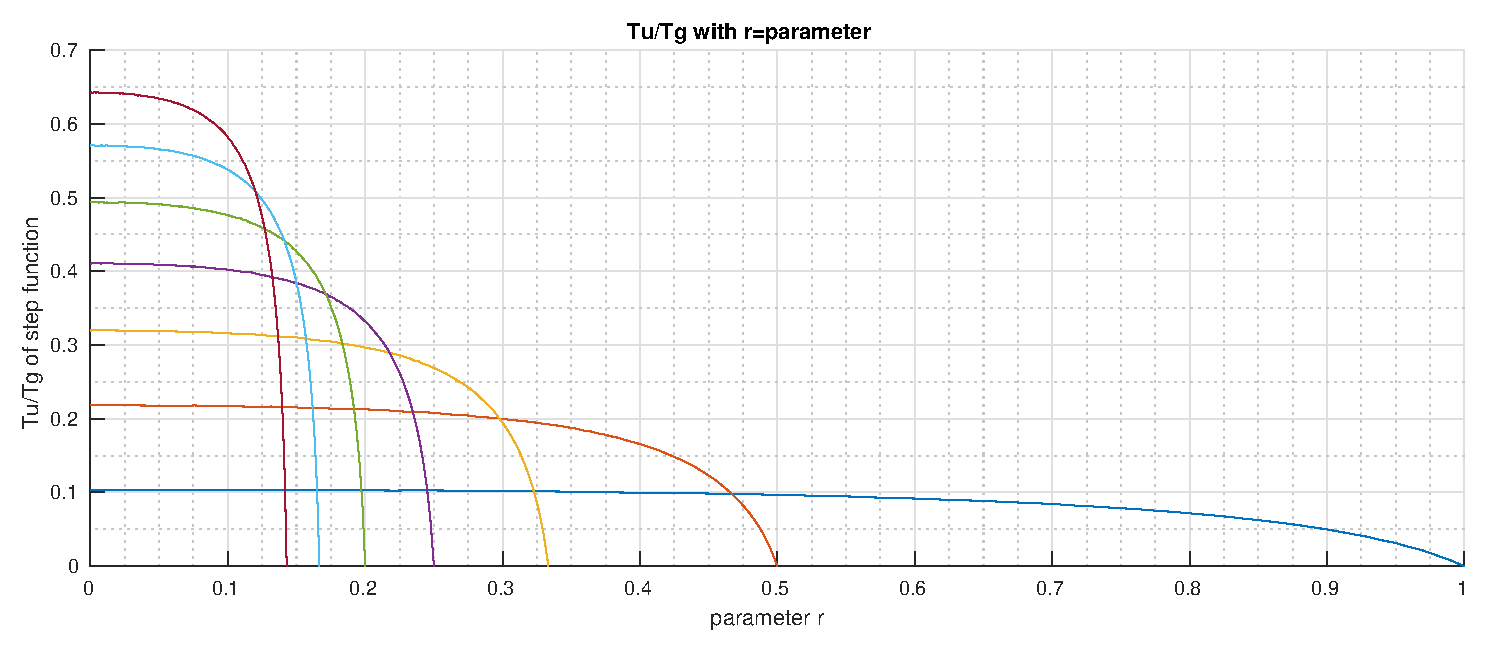
\includegraphics[width=\linewidth]{images/hudzovic_curves_tu_tg}
    \caption{Hudzovic Tu/Tg and 1/Tg lookup curves.}
    \label{fig:hudzovic_tu_tg}
\end{figure}
\begin{figure}
    \includegraphics[width=\linewidth]{images/sani_curves_tu_tg}
    \caption{Sani Tu/Tg and 1/Tg lookup curves.}
    \label{fig:sani_tu_tg}
\end{figure}
\begin{figure}
    \includegraphics[width=\linewidth]{images/hudzovic_curves_t10_t50_t90}
    \caption{Hudzovic (t90-t10/t50) and 1/t50 lookup curves.}
    \label{fig:hudzovic_t3}
\end{figure}
\begin{figure}
    \includegraphics[width=\linewidth]{images/sani_curves_t10_t50_t90}
    \caption{Sani (t90-t10)/t50 and 1/t50 lookup curves}
    \label{fig:sani_t3}
\end{figure}

Visualising   these   functions   yields    the    curves    seen    in   figure
\ref{fig:hudzovic_tu_tg}. What these plots show beautifully is  that  the higher
the order $n$, the steeper -- or more  ``complex''  -- the step response becomes
(smaller values of $T_g$ mean faster rise  times of the step responses). Another
important thing to observe is how lower orders of $G_n(s,r)$ aren't able to rise
as fast as higher orders are able to, \textbf{regardless} of $r$  and  $T$. This
can also be seen in figure \ref{fig:hudzovic_tu_tg},  lower  orders cannot reach
ratios of $T_u/T_g$ that higher orders can.

As discussed earlier, determining the complexity of a step  response is directly
related to the  required  order  $n$  of  the model. Finding $n$ is now a simple
matter  of  computing  $\textrm{plant}_{T_u/T_g}$  and  iterating   through  the
different  curves in figure \ref{fig:hudzovic_tu_tg} until we find an  $n$  that
satisfies the condition:

\begin{equation}
    g_{T_u/T_g}(r, n)\lvert_{r=0} \hspace{2mm} \le \hspace{2mm} plant_{T_u/T_g}
    \label{eq:find_n}
\end{equation}

Ideally,  we'd  like  $n$  to  be  as  small   as   possible,   hence   equation
\ref{eq:find_n}.

With the  parameter $n$ defined, the next step is to find the intersection point
of  $g_{T_u/T_g}(r, n)$ with the horizontal line  $plant_{T_u/T_g}$.  This  will
yield parameter $r$. This can be achieved by solving a simple  line intersection
equation  and  plugging  in  the   locations   of   the  two  horizontal  lines.

The last parameter, $T$, can finally be determined  by  evaluating $g_{1/T_g}(r,
n) \cdot T_g$. Graphically, this equates to finding the  intersection  point  of
the vertical line going through $r$ and the function $g_{1/T_g}(r, n)$ in figure
\ref{fig:hudzovic_tu_tg} and multiplying the result by $T_g$.

